\documentclass{article}%
\usepackage[T1]{fontenc}%
\usepackage[utf8]{inputenc}%
\usepackage{lmodern}%
\usepackage{textcomp}%
\usepackage{lastpage}%
\usepackage[head=40pt,margin=0.5in,bottom=0.6in]{geometry}%
\usepackage{graphicx}%
%
\title{\textbf{María Corina Machado marchó en Barquisimeto contra el Gobierno nacional}}%
\author{MARLA PRATO}%
\date{06/12/2018}%
%
\begin{document}%
\normalsize%
\maketitle%
\textbf{URL: }%
http://www.eluniversal.com/venezuela/27597/maria{-}corina{-}machado{-}marcho{-}en{-}barquisimeto{-}contra{-}el{-}gobierno{-}nacional\newline%
%
\textbf{Periodico: }%
EU, %
ID: %
27597, %
Seccion: %
venezuela\newline%
%
\textbf{Palabras Claves: }%
NO\_TIENE\newline%
%
\textbf{Derecho: }%
CONTEXTO%
, Otros Derechos: %
NO\_TIENE%
, Sub Derechos: %
NO\_TIENE%
\newline%
%
\textbf{EP: }%
SI\newline%
\newline%
%
\textbf{\textit{La coordinadora de Vente Venezuela aseguró que la Asamblea Nacional debe llamar a un gobierno de transición}}%
\newline%
\newline%
%
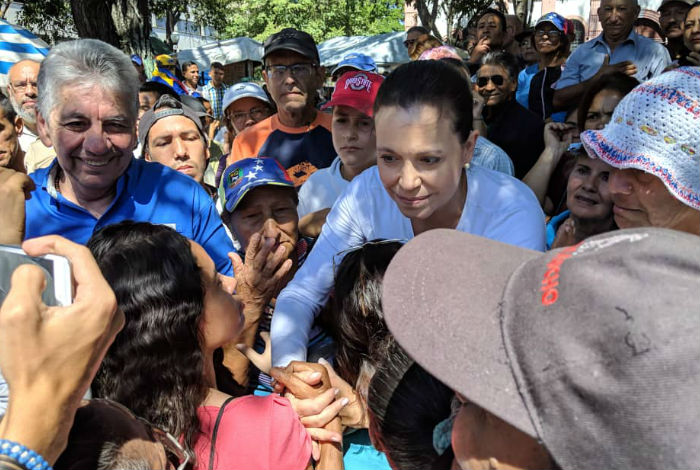
\includegraphics[width=300px]{226.jpeg}%
\newline%
%
Barquisimeto.{-} "Se acabaron las opciones de diálogos, el pueblo ya no puede esperar, la Asamblea Nacional deberá llamar a un gobierno de transición pues ningún gobierno reconocerá a Nicolás Maduro como presidente de Venezuela, y menos el pueblo venezolano", aseguró María Corina Machado, dirigente de Vente Venezuela.%
\newline%
%
Machado, en compañía del exalcalde Alfredo Ramos y representantes sindicales, gremiales y estudiantiles{-} marchó por todo el centro de Barquisimeto para manifestar su rechazo al Gobierno nacional al que calificó de "ilegítimo".%
\newline%
%
A las 11 de la mañana se concentraron en la Plaza San José del centro de la ciudad en donde expresaron que realizaron esta marcha "contra la tiranía, contra la dictadura".%
\newline%
%
Gente de la calle se acercó a saludar a los dos dirigentes y a expresar su descontento ante la grave situación que están viviendo. Pensionados del Banco Bicentenario denunciaron la situación que viven al ir a cobrar sus pensiones y encontrarse que "nunca hay línea ni dinero en las taquillas".%
\newline%
%
"Llevamos más de dos semanas intentando cobrar lo que ha anunciado {-}Maduro{-}" dijo Juan Canelón, quien señaló que "ha sido imposible (cobrar) porque o no hay dinero efectivo, o no hay línea y eso es todos los días".%
\newline%
%
Igualmente comentó sobre "las interminables colas" que se hacen en los alrededores de los bancos que obliga a los adultos mayores a dormir en las aceras y la calle durante días "para ver si cobran algo".%
\newline%
%
Durante el recorrido Machado y Ramos saludaron a la gente y estrecharon las manos de los funcionarios policiales apostados a lo largo de la avenida para resguardar y ofrecer seguridad en la zona, así como a los que resguardan el edificio sede de la gobernación del estado.%
\newline%
%
Muestras de apoyo y al grito de consignas como “Maduro fuera”, “abajo la tiranía”, “Maduro ilegitimo” “dictador” recorrió la marcha las calles del centro mientras muchas personas aplaudían al paso de los dirigentes políticos.%
\newline%
%
Machado sostuvo que la fracción del 16J tiene "el compromiso" de llamar a un Gobierno de transición en las próximas semanas porque, a su juicio, la población "ya no puede esperar más ante la crisis en la que los ha sumergido este Gobierno déspota y tiránico".%
\newline%
%
Por su parte, Alfredo Ramos sostuvo que las condiciones de este país "no están para estar celebrando elecciones".~Esto {-}dijo{-} "es un parapeto para ganar tiempo y hacer creer que hay democracia en el país y eludir la compleja situación".%
\newline%
%
En horas de la tarde la coordinadora de Vente Venezuela asistió a un foro que tuvo lugar en el Salón Amazonía en el centro de la ciudad.%
\newline%
%
\end{document}